\documentclass[a4paper,10pt]{article}
\usepackage[utf8]{inputenc}
\usepackage{amssymb}
\usepackage{fullpage}
\usepackage{verbatim}
\usepackage{multirow}
\usepackage{csquotes}
\usepackage{tikz}
\usepackage[T1]{fontenc}
\usepackage{lmodern}
\usepackage{lscape}
\usetikzlibrary{arrows, arrows.meta, fit,positioning,shapes,automata}
\usepackage{fancyhdr}
\usepackage[titletoc,title]{appendix}
\usepackage[hidelinks]{hyperref}%
\usepackage[section,numberedsection, acronym, toc]{glossaries}
%\newacronym{grant}{GRANT}{Global Resource Allocation via Network Topology}
\makeglossaries
\bibliographystyle{apalike}

\longnewglossaryentry{global resource allocation by network topology (GRANT)}
{name=global resource allocation by network topology (GRANT)}{a strategy to allocate service tasks in a balanced way.}
\longnewglossaryentry{finger pointing}{name=finger pointing}{litigation scheme allowing upstream peers to shift blame to downstream peer"}
\longnewglossaryentry{certified delivery}{name=certified delivery}{message delivery with signed receipt from recipient}
\longnewglossaryentry{object stream}{name=object stream}{series of messages passed from one node to its peer}
\longnewglossaryentry{handover state}{name=handover state}{root hash of an outgoing data stream signed against downstream peer and time}
\longnewglossaryentry{takeover state}{name=takeover state}{handover state signed against initial state by downstream peer}
\longnewglossaryentry{provable data exchange}{name=provable data exchange}{peer to peer object streams allowing handover and takeover proofs}
\longnewglossaryentry{kademlia topology}{name=kademlila topology}{a scale free network topology that has guaranteed path between any two nodes in $O(log(n))$ hops}
\longnewglossaryentry{request and disappear}{name=request and disappear}{property of warranted service provision networks, whereby a service task request gains service guarantees in a single instant swap exchange}
\longnewglossaryentry{mutable resource update notifications}{name=mutable resource update notifications}{}
\longnewglossaryentry{resource update chunk}{name=resource update chunk}{}
\longnewglossaryentry{forwarding kademlia}{name=v}{}
\longnewglossaryentry{scale-free graphs}{name=}{scale-free graphs}
\longnewglossaryentry{kademlia}{name=}{kademlia}
\longnewglossaryentry{kademlia table}{name=kademlia table}{}
\longnewglossaryentry{kademlia topology}{name=kademlia topology}{}
\longnewglossaryentry{retrieve request}{name=retrieve request}{}
\longnewglossaryentry{proximity order}{name=proximity order}{}
\longnewglossaryentry{proximity bin}{name=proximity bin}{}
\longnewglossaryentry{neighbourhood}{name=neighbourhood}{}
\longnewglossaryentry{radius of responsibility}{name=radius of responsibility}{}
\longnewglossaryentry{retrievability}{name=retrievability}{}
\longnewglossaryentry{redundant retrievability}{name=redundant retrievability}{}
\longnewglossaryentry{practical retrievability}{name=practical retrievability}{}
\longnewglossaryentry{consistent retrievability}{name=consistent retrievability}{}
\longnewglossaryentry{synchronisation}{name=synchronisation}{}
\longnewglossaryentry{historical sync state}{name=historical sync state}{}
\longnewglossaryentry{live sync state}{name=live sync state}{}
\longnewglossaryentry{chunk}{name=chunk}{}
% \longnewglossaryentry{}{name=}{}
% \longnewglossaryentry{}{name=}{}
% \longnewglossaryentry{}{name=}{}
% \longnewglossaryentry{}{name=}{}
% \longnewglossaryentry{}{name=}{}
% \longnewglossaryentry{}{name=}{}
% \longnewglossaryentry{}{name=}{}
% \longnewglossaryentry{}{name=}{}
% \longnewglossaryentry{}{name=}{}


\newcommand\gloss[1]{\emph{\gls{#1}}}


\title{Decentralised peer-to-peer network for route}
% \subtitle{Scalable infrastructure for decentralised service economies}
\author{Viktor Trón, Aron Fischer, Daniel A. Nagy}
\date{\today}
\begin{document}


\maketitle
% \begin{abstract}
% \end{abstract}

\setcounter{tocdepth}{2}
\tableofcontents
\section{Message relaying and routability}
\label{sec:relaying}

In this section we describe how a network of nodes can use an overlay topology to support messaging between arbitrary nodes using overlay addressing. We explore conditions of routability.

\subsection{Overlay topology}



\subsubsection{Scale free graphs}
\subsubsection{Logarithmic distance and proximity order}

Consider the set of byte sequences with fixed length $l$ as points in a space. We can define a distance metric $\delta$ such that
the distance between two equal-length byte sequences is defined as the bigendian  numerical value of their bitwise XOR ($\xor$).

$$
\delta(x, y) = \mathit{Uint}(x  \xor y)
$$

Given the fixed length $l$, there is a maximum distance in this space, and thus we can define an `inverse' distance or \gloss{proximity}:

$$
\pi(x,y) = \delta_{\mathit{max}}-\delta(x, y), 
$$

where

$$
\delta_{\mathit{max}} = 2^l-1
$$

\emph{Proximity order} is a discrete logarithmic scaling of proximity.
It is defined as the reverse rank of the integer part of the base 2
logarithm of the distance.


$$
\mathit{PO}(x,y) = l-\mathit{int}(\log_2(\delta(x, y)))
$$


In practice, $\mathit{PO}(x,y)$ is calculated by counting the number of common leading zeros in $x \xor y$, .

Taking the \gloss{proximity order} relative to a fixed point $x_0$ partitions the points in
the space (of byte sequences of length $l$) into discrete bins. Points in each bin are at
most half as distant from $x_0$ as items in the previous bin. Furthermore, any two addresses belonging to the same bin are at most half as distant from each other as they are from $x_0$, or in terms of proximity order:

$$
\text{for every node } x \text{ and target address } t, \text{ such that} \mathit{PO}(x_0, t) = \mathit{PO}(x_0,x) 
$$

$$
\mathit{PO}(x, t) > \mathit{PO}(x_0, t) 
$$


Consider a set of points in the space and 
a binary relation $R$. Define a graph where every point in the set is a vertex and any two vertices $x$ and $y$ are  connected with an edge if they are in relation $R$. 

Points that are in relation $R$ with a particular point $x_0$ can be indexed by their proximity order relative to $x_0$. 
This can serve as the basis for local decisions in graph traversal where the task is to find a path between two
points. 

We say that a node has \emph{kademlia connectivity} if (1) it is connected to at least one node for each proximity order up to (but excluding) some maximum value $d$ (called the \gloss{saturation depth}) and (2) it is connected to all nodes whose proximity order relative to the node is  $\geqslant d$.

If each point of a connected subgraph has kademlia connectivity, then we say the subgraph has a \gloss{kademlia topology}. In a graph with kademlia topology, (1) a path between any two points exists, (2) it can be found using only local decisions on each hop and (3) is guaranteed to terminate in no more steps than the depth of the destination plus one. 

The procedure is as follows. Given point $x$ and $y$, construct the path $x_0=x , x_1, ..., x_k=y$ such that $x_{i+1}\in \mathit{PO}(x_i, x_{i+1})=\mathit{PO}(x_i, y)$, i.e., starting from the source point, choose the next point from the PO bin that the destination address falls into: because of the assumption of kademlia connectivity (1) such a point exists. Due to our previous conjecture, the actual bin is monotonically increasing at each step and can start with zero, therefore for every $0<i<=l$, $\mathit{PO}(x_{i}, y)>=i$. So there exists a $d<=d_y$, such that 
$\mathit{PO}(x_{d}, y)>=d_y$, which together with kademlia connectivity criterion (2) entails that either $x_d=y$ and $k=d$, or $y$ is connected to $x_d$, so we can choose $x_{d+1}=y$, and $k=d+1<=d_y+1$.

Given a set of points uniformly distributed in the space (e.g., the results of a hash function applied to swarm data) the proximity bins map onto a series of subsets with cardinalities on a negative exponential scale, i.e., PO bin 0 has half of the points of any random sample, PO bin 1 has one fourth, PO bin 2 on eighth, etc.
The expected value of saturation depth in the network is $\log_2(N)$. The last bin can just merge all bins deeper than the depth and is called the \gloss{most proximate bin}.

\subsubsection{Flavours of Kademlia routing}
\label{sec:kademlia} 

The properties of a kademlia graph can be used for routing messages between nodes in a network using overlay addressing. Nodes in the swarm network are identified by the hash of the ethereum address of the swarm base account. This serves as their overlay address, the proximity order bins are calculated based on these addresses. 

In the following we apply kademlia graph properties to nodes in an overlay network. In particular we show that two relations over nodes can be used to support two flavours of routing, \emph{iterative} and \emph{recursive}.


For instance, take $R$ as the 'know about' relation:
$x$ 'knows about' $y$ if $x$ has both overlay and underlay address information on $y$. 


Peers known to any particular node $x$ can be indexed by their proximity order relative to $x$. This is called the \gloss{kademlia table} of the node (see figure \ref{fig:kademliatable}). 
Node $x$ has a \gloss{saturated kademlia table} if there is a $0<=d_x<=l$ such that (1) the node has at least one peer in each bin up to and excluding PO $d_x$ and (2) all peers at least as near as $d_x$ are known to $x$. 
If each node in a set has a saturated kademlia table given $R$, then $R$ has kademlia topology.


The iterative kademlia routing the requestor node iteratively extends its 'know-about' graph. Using their underlay address (usually UDP) contact their direct peers for further peers, on each successive iteration the peer is at least one order closer to the destination. Because of kademlia criteria, the requestor will end up knowing about the destination node's underlay address and can communicate. This iterative strategy%
%
\footnote{The iterative protocol is equivalent to   the original kademlia routing that is described in \cite{maymounkov2002kademlia}.
}
%
critically depends on the nodes' ability to find peers that are online. In order to find one, a node needs to collect several candidate peers for each bin. The best predictor of availability is the recency of the peer's last response, so peers in a bin should be prioritised according to this ordering.




\begin{figure}[htbp]
   \centering
   \caption{Kademlia table:  peers of node $x$ partitioned into proximity order bins. Saturated kademlia connectivity is 
   characterised by a live kademlia table of directly connected TCP peers such that (1) there is at least $k$ peers in each bin up to but excluding saturation depth $d_x$ and (2) no peers in the entire network that are not in the node's most proximate bin $d_x$. }
   \label{fig:kademliatable}
\end{figure}

An alternative flavour of kademlia routing is described in \cite{heep2010r}. Here, a recursive method is employed, whereby the successive steps of the iteration are outsourced to a downstream peer.
Each node recursively calls a direct peer to pass a message to the destination. If kademlia routing is used, this directly translates to relaying messages via a chain of peers ever closer to the destination.

Swarm uses the ethereum devp2p rlpx  as the underlay transport. This uncommon variant allows semi-stable peer connections (over TCP), with authenticated, encrypted, synchronous data stream. Peers connected to a node define another, \emph{live} kademlia table, 
where the graph edges represent devp2p rlpx connections. 
The two criteria of healthy kademlia connectivity translate as: for each node $x$, there exists a $d_x$ such that (1) the node $x$ is connected to at least one peer for each PO bin up to but excluding      $d_x$ and (2) connected to all the nodes at least as near as $d_x$.
If each node in a set has a saturated kademlia table of connected peers, then the nodes `live connection' graph has kademlia topology.
Since one does not need to select peers that are online, the recursive step consists solely of forwarding the message to a connected peer strictly closer to the destination. We can call this alternative \gloss{forwarding kademlia}. 

In a forwarding kademlia network, a message is said to be \emph{routable} if there exists a path from sender to destination through which the message could be relayed. 
In a mature subnetwork with kademlia topology every message is routable. 


A message is said to be \emph{practically routable} if it can be routed to its destination within the typical timeframe of a request. If all peer connections are stably online, all routable messages are practically routable. It is expected however, that a large proportion of nodes are not stably online. Keeping several connected peers in each PO bin, each node can guarantee that it can forward any message at any point in time, even if their peer drops after the message is received but before it is forwarded. Healthy nodes could commit to being able to forward within a (very short) time we can call \emph{forwarding lag}. In case a downstream peer disconnects before this forwarding lag passes, then upstream peers can reforward the message to an alternative peer, thereby keeping the message passing unbroken. 

In a stable network with stable connectivity, a slim kademlia table, i.e., one peer for each bin up to $d$, is sufficient to guarantee routing between nodes.
However, to guarantee \gloss{practical routability}, it is best to keep several connections in each bin (see also section \ref{sec:bindensity}) so that the kademlia table remains saturated even if there are disconnections. Given a model of node dropouts, we can calculate the minimum number of peers needed per bin to guarantee that  nodes are saturated $x\%$ of the time.

\subsection{Bootstrapping and discovery}
\label{sec:bootstrapping} 

This  section discusses how a stable kademlia topology  can emerge. 
In particular, what is the exact bootstrapping protocol each node  needs to follow to reach a redundantly saturated kademlia connectivity and maintain it. Nodes joining a decentralised network  are supposed to be  naive, i.e., potentially connect via a single known peer. For this reason, the bootstrapping process  will need to include a discovery component with the help of which nodes exchange information about each other.  

The protocol is as follows:
Initially, each node has zero as their saturation depth. Nodes keep advertising their saturation depth as it changes to their connected peers. If a node establishes a new connection, it notifies each of its peers about it if the new connection's proximity order relative to the respective peer is not lower than the peer's advertised saturation depth. The notification is always sent to each peer that shares a PO bin with the new connection.  Formally, $x$ notifies $p\in\mathit{PeersOf}(x)$ of its new connection to $y$ if $\mathit{PO}(x, p) = \mathit{PO}(x, y)$ or $d_p <= \mathit{PO}(y, p)$. In particular, notification contains  full overlay and underlay address information.%
%
\footnote{Light nodes that do not wish to relay messages and do not aspire to build up a healthy  kademlia are discounted, see section \ref{sec:light}. }

As a node is being notified of new peer addresses, it stores them in  a kademlia table of known peers. 
While it listens to incoming connections, it also proactively attempts to connect to nodes in order to achieve saturation: it tries to connect to each known node that is within the PO boundary of $n$ nearest neighbours ($nd$, \gloss{nearest neighbour depth}) and (2) it tries to fill each bin up to $nd$ with healthy peers. To satisfy (1) most efficiently, it attempts to connect to the peer that is most needed at any point in time. Low (far) bins are more important to fill than high (near) ones since they handle more volume. Filling an empty bin with one peer is more important than adding new peer to a non-empty bin, since it leads to a saturated kademlia earlier. Therefore the protocol uses a \emph{bottom-up, depth-first strategy} to choose a peer to connect to.  Nodes that are tried but failed to get connected are retried after a time interval that doubles after each attempt. After a certain number of attempts such nodes are no longer considered.

After a sufficient number of nodes are connected, a bin becomes saturated, and the bin saturation depth can increase.
Nodes keep advertising their current saturation depth to their peers if it changes. 
As their saturation depth increases, nodes will get notified of fewer and fewer peers. Once the node finds all their nearest neighbours and has saturated all the bins, no new peers are expected. For this reason, a node can conclude  a saturated kademlia state if it receives no new peers (for some time).%
%
\footnote{The node does not need to know the number of nodes in the network. In fact, some time after the node stops receiving new peer addresses, the node can effectively estimate the size of the network: $\log_2(n+1)+ nd$}
%
Instead of having a hard deadline and a binary state of
saturation, we can quantify certainty of saturation by the age of the last new peer received.

When there are no new peers received for a while and all bins are saturated, the node notifies its peers of the \gloss{age of saturation} (the time the last new peer was received). If the node receives a new peer after this, peers are notified again.

Assuming stable connections, eventually each node online will get to know its nearest neighbours and connect to them while keeping each bin up to $nd$ non-empty. Therefore each node will converge on the saturated state. 
After a node and all its peers have been saturated for a while, the node can advertise \gloss{age of health}, 
that is the time of the most recent age of saturation among all the saturated peers. 

If no new nodes join, health (kademlia topology) is maintained even if peer connections change. A node is not supposed to go back to a lower saturation state for instance. This is achieved by requiring several peers in each PO bin. 
If new peers do arrive, all nodes reissue the age of saturation and reset the age of health. The delay before advertising saturation should be long enough so that this regression of state only happens in case there is actually a new node joining the network.


\subsection{Incentivisation of relaying}

This section explores how to incentivise nodes to keep healthy connectivity and forward messages. We discuss how reward schemes and punitive measures achieve varying degrees of delivery guarantee.

\subsubsection{Compensation for relaying}

In order to incentivise relaying nodes a message relaying fee needs to be introduced.  We stipulate that the relaying fee for passing one message to a direct peer is proportional to the number of PO bins that the hop spans. Relaying fee is accounted for as part of \gloss{swap} (swarm accounting protocol). The simple rational strategy to maximise profit will incentivise nodes to find the closest node to the destination when relaying as well as maintain a healthy connectivity needed for successful profitable routing. Furthermore, the entire message delivery fee $\phi$ can be precalculated as the expected PO span the message needs to travel and can be offered by the sender. 

Assume $x$ wants to send a message to $y$, then finds a peer $x_1$ in $y$'s bin, and offers a fee
$\phi_0 = E(d)-\mathit{PO}(x, y)$ units to $x_1$. Assume $x_1$ forwards to $x_2$ then it needs to pay $\phi_1=E(d)-\mathit{PO}(x_1, y)$. The net profit for $x_1$ is the difference between the upstream fee it charged and  the downstream fee it pays, ie., $p=\mathit{PO}(y, x_2)-\mathit{PO}(y, x_1)$ which is proportional with the number of PO bins the message got closer to $y$. The more nodes there are in a bin, the more likely, a node can choose $x_2$, such that  $p$ is highest.       

This presupposes that nodes do forward the message though. The most basic possible attack vector is that a malicious node takes over messages but does not forward them. Such a malicious node has no downstream peer to pay to so it takes swap revenue for the entire PO span to the destination. If relay fees due to downstream peers are accounted for at the time the request is taken up, there is no going back even if the message fails to arrive. This in itself is not a problem since the forwarding fee is minuscule. As long as the the node that broke the chain can somehow be detected. 

Peers can agree that every message is responded to with an acknowledgement signed by the destination. If
this is passed back the same route along which the original message was forwarded, peers can agree to pay for the swap at the time the delivery is acknowledged. This positively rewards relaying and makes withholding not profitable. 
Lack of evidence that the message did arrive can just be used to prompt sender to resend. With some extra administrative overhead the conditional payment can be implemented as a bounty specifying proof of delivery as its escrow condition. This construct would prevent nodes to ever charge for non-delivered messages which is a dubious gain given that the profit to be gained before detection makes this attack unlikely. 
This scheme of \gloss{certified delivery} can be strengthened to \gloss{guaranteed delivery} with the help of a provable data exchange. 
 
\subsubsection{Provable data exchange} 

Assume that two nodes participate in a particular service that involves relaying objects. The content addresses (swarm hash) of consecutive objects sent in one direction constitute a \emph{data stream}. Both peers save this stream to swarm and maintain an up-to-date index (say of hashes to offsets) according to some predefined ruleset. The upstream peer (sender) calculates the swarm hash of this index and periodically signs it against the current blockheight or timestamp as well as the data stream identifier. This \gloss{handover state} is periodically sent to the downstream peer (receiver) who verifies it and preserves it until the next one. The downstream peer periodically countersigns the handover state together with an initial offset or timestamp. This \gloss{takeover state} is then sent to the upstream peer. For instance, the handover state obtained from the upstream peer can be used to prove to third parties that an object X was handed over to the downstream peer. This can be done by giving an inclusion proof of the hash of X in the current index signed in the takeover state.%
%
\footnote{Upstream peer can be challenged to give this inclusion proof.}

\subsubsection{Delivery guarantees} 

Rewards given to relayers as part of swap can give reasonable incentives for correct delivery especially if swap accounting is done with certified delivery acknowledgements used as invoice. 

Such a scheme assumes certified delivery acknowledgements can be used as escrow conditions for conditional bonds. 
% weak guarantees
If the  bond is conditioned on some signed acknowledgment obtained from the destination address to release the delivery fee, then each node on the way is incentivised to forward the message. 


On top of the reward peers get for relaying, we can introduce additional incentives to guarantee that messages reach the recipient. We can assume that relaying nodes  promise to relay messages in a data stream towards the recipient by registering on a service contract. If registration involves a locked stake, and thus registered nodes have a stake to lose, then punitive measures can be imposed on nodes that fail or refuse to relay messages in the data stream.

Take the example of A sending a message to remote node D, and assume that B, C, and D are all registered relaying nodes that are online. If there is reason to believe that the message did not reach D, A can challenge B by simply providing the takeover proof for the message. B can defend itself by providing takeover proof from C, thereby shifting the blame to C for blocking the delivery. C in turn can show takeover proof from D to refute the challenge. It can also happen that C indeed did not forward the message because there was no node closer to D among its peers. But this means that D is a nearest neighbour of C, in which case D should have been connected to C.
Therefore D can be challenged to prove that it was connected to C. D can respond to the challenge
by showing handover state obtained from C dated after the message delivery deadline. This in turn is
a challenge to C to show the inclusion proof of the message against the handover state.
This pattern is called \gloss{finger pointing} and constitutes the investigative part of litigation which results in identifying the node ultimately responsible for failed delivery by not relaying. Finger pointing essentially implements \emph{guaranteed delivery}.

This scheme of guaranteed delivery requires nodes not to be offline for longer than their last non-relayed message's expiry. 
By virtue of taking over a message to relay, nodes commit to staying online until the corresponding conditional bond expires (message delivery deadline). 
Practically, in order to respond to a challenge, nodes need to be online for an extra grace period during which finger pointing litigation is valid. 

In this section, we introduced a forwarding kademlia network with overlay addressing. We showed that if nodes have a redundantly saturated kademlia table, then every message is practically routable in logarithmic hops using local decisions on nodes.
We showed how certified delivery acknowledgments allow nodes to detect if a message was not relayed. Weak delivery guarantees can be obtained with payments conditional on receipt. Stronger delivery guarantees require nodes to register on the blockchain with a stake and use provable data exchange to enable finger pointing litigation. 

\section{Chunk storage and retrievability}

In this section we explain how a  kademlia overlay network can be used as a distributed chunk store and content distribution network. We explore conditions of retrievability.

\subsection{Using kademlia network for storage}

\subsubsection{Distributed hash tables}
 
Distributed hash tables (DHTs) utilise an overlay network to implement a key-value store distributed over the nodes. The basic idea is that the keyspace is mapped onto the overlay address space, and information about an element in the container is to be found with nodes whose address is in the proximity of the key. In the simplest case, let us say that the closest node to the key stores the value. 
All flavours of kademlia are perfectly suited to serve as routing data requests in the DHT. 

\subsubsection{Content addressing and distributed preimage archive}

DHTs for decentralised content address storage typically associate content fingerprints with a list of nodes (seeders) who can serve that content \cite{ipfs2014}. However, the same structure can be used directly: it is not information about the location of content that is stored at the node closest to the address (fingerprint), but the content itself. We call this structure \gloss{distributed preimage archive} (DPA). 

A DPA is opinionated about which nodes store what content and this implies a few more restrictions. (1) load balancing of content is required among nodes and is realised by splitting content into equal sized chunks (\gloss{chunking}). (2) there has to be a process whereby chunks get to where they are supposed to be stored (\gloss{syncing}); and (3) since nodes do not have a say in what they store, measures of \gloss{plausible deniability}  should be employed. 


\subsubsection{Mutable resources and resource update archive}

Resource updates are chunks but validating them does not involve checking the swarm hash of the content against the address. 

\subsection{Retrievability}


\subsubsection{Chunk retrieval and routability}

In a distributed chunk store, a chunk is said to be \emph{retrievable} for a  requestor node if it can reach a storer node and have the content delivered using the content address only.
In section \ref{sec:relaying}, we introduced swarm as a semi-stable peer to peer network with forwarding kademlia overlay routing. f    
So given a fixed DPA with healthy kademlia overlay topology, every chunk  is retrievable to every node.

A chunk is said to be \emph{practically retrievable} if a path can be found for requests and deliveries given the typical connectivity changes of the swarm network within the typical timeframe of requests. 
It is expected that a large proportion of swarm nodes are not stably online. Such a high churn situation is problematic if we use the naive strategy of forwarding requests to any one closer node. If a node on the path drops offline during the request-delivery roundtrip, the forwarding is broken, effectively rendering the chunk requested not practically retrievable. 

For this reason alone forwarding requests to any one closer node is not viable. Assuming that (1) the node closest to the chunk address has the chunk data and (2) the nodes along the request route remain online, the strategy of forwarding along healthy kademlia nodes ensures practical retrievability.
However, both of these assumptions are unrealistic. Provided the requests contains the address of the requestor, (2) can be relaxed to a weaker assumption that the network has stably healthy kademlia topology (although nodes can come and go). For retrieve requests, nodes use the chunk address as destination, whereas  for the delivery, they use the requestor address as destination if the intermediate peer requestor is no longer connected. 
In this case, the delivery of the chunk can potentially travel a  route different from the request. As long as there is healthy kademlia topology and the destination is known, paths (with number of hops logarithmic to the network size) are guaranteed to be found in both directions. 
This effectively means that chunk retrieval with anonymous requests will need to resort to other tools to guarantee practical retrievability (see section below). 


\subsubsection{Redundancy by local replication}

As for (1), high churn is even more problematic: if the closest node is the only storer and drops out, there is no way to retrieve the content. This basic scenario is handled by having a set of nearest neighbours holding replicas of each chunk that is closest to any of them. To know the size of the nearest neighbour set and guarantee that chunks are replicated, nearest neighbours should be fully connected. 

A chunk is said to be \emph{redundantly retrievable} of degree $n$ if it is retrievable and would remain so after any $n-1  $ responsible nodes leave the network. The naive approach presented above can be interpreted as degree zero retrievability.
In the case of request forwarding failures, one can retry, or start concurrent retrieve requests. 
Such fallback options are not available if all the storer nodes go down. Therefore redundancy is of major importance.


The area of the fully connected neighbourhood defines an \gloss{area of responsibility}. 
Since storer nodes in the nearest neighbourhood synchronise all chunks they have, a storer node must store each chunk whose address falls in the area of responsibility. The PO boundary of the area of responsibility (nearest neighbours depth) defines a \gloss{radius of responsibility} for the node. 

A storer node is said to be \emph{responsible} for (storing) a chunk if the chunk address falls within the node's radius of responsibility.
Let us assume then (1) the forwarding strategy that relays requests along stable nodes and (2) the storage strategy that each node in the nearest neighbourhood (of $R$ nodes) stores all chunks the address of which fall within the radius of responsibility. As long as these assumptions hold, each chunk is retrievable even if $R-1$ storer nodes drop offline simultaneously. As for (2), we still need to assume that every node in the nearest neighbour set can store each chunk.
Realistically, however, a large proportion of (even stable) nodes will potentially have resource limitations.
Since with time, the overall amount of distinct chunks ever uploaded to swarm will increase indefinitely, such resource limitations will need to be explicitly addressed. 
As a result, the naive strategy of choosing the nearest $R$ saturated kademlia peers to determine the radius of responsibility is not viable.


\subsubsection{Storer nodes and relaying nodes}

A further distinction within stable nodes is needed: between \gloss{storer node} and  \gloss{relaying node}.
When counting effective peers to saturate a kademlia bin, relaying nodes are good candidates as they can forward retrieve requests and even serve chunks that are popular and recent if they turn on caching. 
Since they cannot guarantee storing all chunks in their neighbourhood, however, relaying  nodes should not count when calculating the radius of responsibility. 

Relaying nodes are recognised by relaying requests of chunks that belong in their area of responsibility (potentially to a node that is farther from requested chunk than the node itself). Nodes that cannot store all chunks they are responsible for cannot be storer nodes. While they can misadvertise themselves as a storer node towards farther peers and as a result receive retrieve requests, they need to serve these requests. However, if they fail to provide chunks that are in their radius of responsibility as guessed by their peers, they risk reputation long term. Therefore relaying nodes have the incentive to connect to a storer node to which they will forward retrieve requests. In this case, however, they are recognised by their nearest neighbours as non-storer nodes who can therefore correctly calculate their radius of responsibility which we define as follows:

$$
\mathit{RR(x)} = \max_r(|\{y\in \mathit{Kad}(x): \mathit{PO}(x, y)>=r\}| >= R)
$$

Following the bootstrap strategy in section \ref{sec:relaying} we saturate a node $x$'s kademlia table with at least $m$ storer peers in each PO bin, arriving at a saturation depth $d$. The redundancy parameter $R$ determines the minimum cardinality of the nearest neighbour set. 

\subsection{Eventual consistency and chunk syncing}

In this section we discuss the criteria of \gloss{eventual consistency} and show how it can be achieved by syncing chunks and advertising sync status.

If no storage or bandwidth constraints are encountered, any chunk uploaded to any node should become retrievable within a short time. No amount of new nodes joining the network should be able to cause a retrievable chunk to stop being retrievable. If no nodes leave the network and no new chunks are uploaded, all chunks stored by any of the nodes should become retrievable over time.



\subsubsection{History and session syncing}

When two nodes connect and they engage in synchronisation, the upstream node offers all the chunks it stores locally in a datastream per proximity order bin. To receive chunks closer to a downstream than to the upstream, downstream peer subscribes to the data stream of the PO bin it belongs to in the upstream node's kademlia table.
If the peer connection is within nearest neighbour depth the downstream node subscribes to all PO streams $nd<=i<=\mathit{maxPO}$, ie., the most proximate bin. Calculating $nd$ is not trivial though. 

Nodes keep track of when they stored a chunk locally for the first time (for instance by indexing them by an ever incrementing storage count). The downstream peer is said to have completed \gloss{history syncing}, or is \emph{history synced} if it has (acknowledged) all the chunks of the upstream peer up from the beginning until the time the session started (up to the storage count that was the highest at the time the session
started). Note that due to disk capacity limitations, having synched all chunks does not mean that the node can store all the chunks. In fact, chunks  synced earlier will be garbage collected to make space for chunks synced more recently. If chunks are synced in order of storage this may not result in the node having the most profitable (most often requested chunks). Thus it may be advisable to sync chunks staring with the most popular ones according to upstream peers and finish syncing when storage capacity is reached. This way, a node's limited storage will be optimised. 


Some node $B$ is said to have completed \gloss{session syncing} or is \emph{session synced} with its upstream peer $A$, if each chunk put in $A$'s storage since the session started is also stored in $B$'s storage (or was and got deleted and forwarded since). Given a constant influx of new chunks, the session-synced state for a peer connection is not long lasting. A good measure of the completeness of session synchronisation of a peer connection is given by the recency of the latest session synced state of the downstream peer called \gloss{sync lag}. The more recent the state, i.e., the shorter the sync lag, the more requests the node can serve successfully. 

\subsubsection{Bootstrapping nearest neighbourhoods}

If the overall storage capacity of swarm $C$ is less than the total volume of chunks to be stored ($V$), then not all chunks are retrievable. The ratio of the two gives us an upper limit on the degree of redundancy $R_{\mathit{max}} = \mathit{int}(C/V)$ in a mature swarm.
Let us assume that $R$ is a positive integer, meaning all chunks can be stored with replication factor $R$.

If a node's storage is full with chunks within its radius of responsibility before it gets fully synchronized, it cannot participate as a full storer node in Swarm.
Nodes that store all chunks in their area of responsibility will count as storer nodes. A node can only hope to satisfy this if they have storer nodes in each of their PO bins and they completed history syncing with all of them. Chunks, however, can arrive from nearest neighbours so determining storer status is not immediately straightforward. 
If it was known that each of a node's nearest neighbours is synced with all their respective non-nearest neighbours, then after completing historical syncing with these neighbours, the node may conclude that they are full storer nodes with a particular radius of responsibility. Any nearest neighbour subsequently fully history synced with such a node can also conclude their full storer status. 

In order to kickstart this process, prospective storer nodes advertise their statuses in 3 stages: (1) prospective (2) externally synced with radius of responsibility $r$ (3) externally and internally synced with radius of responsibility $r$.
Nodes advertising (1) are expected to announce (2) after some time (maximum sync delay). 
Nodes advertising (2) count each other as potential nearest neighbours and aspire to synchronise with $R$ of them. If they succeed while maintaining (2) they can advertise status (3). Nodes with full history synced status (3) can advertise as storer nodes.  If a neighbourhood has $R$ storer nodes in it, then every chunk in the neighbourhood is redundantly retrievable to degree $R-1$. The swarm is said to be \emph{mature} if each node has a neighbourhood of $R$ storer nodes.%

Barring storage capacity constraints, following this process of setting the radius of responsibility, and synchronising, nodes are  guaranteed to arrive at chunk distribution where each chunk is redundantly retrievable with degree $R$.

\subsubsection{Capacity constraints}

As mentioned earlier, as the number of distinct chunks ever uploaded will increase. Unless the total storage capacity steadily increases, we should expect that the swarm is able to store only a subset of chunks. There will be nodes that cannot be responsible for all the chunks within their radius of responsibility. 


\subsubsection{Incentives}

Serving chunks in swarm is incentivised with a reward the swap protocol \cite{ethersphere2016sw3}. 
Nodes that serve or relay retrieve requests share an interest that chunks are retrievable. 
This implies that nodes are incentivised to accept and pass on retrieve requests, as well as accept and pass on chunks (syncing) even though they only get compensated for chunk deliveries. 
On the other hand, leaving retrieve requests costless, nodes will be inclined to forward retrieve requests to multiple closer peers in order to reduce latency. Since this always triggers an exponential flooding,  retrieve requests should require a forwarding fee to make concurrent requests the more expensive option. We stipulate that forwarding retrieve requests is analogous to message forwarding and handled with the swap protocol. Alternatively, we can incur the charge when the chunk is delivered.

Nodes receive a reward every time they serve a chunk, therefore the profitability of a chunk is proportional to its popularity: the more often a chunk is requested, the higher the reward relative to the fixed cost of storage per time unit.
When nodes reach storage capacity limits and it comes to deciding which chunks to delete, the optimal strategy of a rational profit maximising agent is to remove chunks whose profitability is lowest. The best predictor for this is the age of last request. In order to maximise the set of chunks to select from, nodes engage in opportunistic caching of the deliveries they relay as well as the chunks they sync. This results in popular chunks being more widely spread and faster served, effectively making the entire swarm an auto-scaling and auto-balancing content distribution network.

Syncing, i.e., the movement of chunks when they are relayed towards their PO custodians can remain free since it is in the interest of both parties with identical risk. 

After building up a healthy kademlia connectivity, and session syncing with their peers, both relaying nodes as well as storer nodes periodically advertise their maximum sync lag, that is the oldest session synced status over all their peers. When a node advertises their max sync lag, they claim that they store all chunks within their radius of responsibility that is older than their sync lag.

If a node has good bandwidth and efficient local storage, they have a better chance of achieving session synced state than nodes having constraints on these resources. History synced status, on the other hand, requires a lot of storage space. So the two types of synchronisation are achieved by potentially different node types. For instance, a node with only memory store and high bandwidth can serve recent chunks earlier than its  fully history synced neighbour. When a storer node receives a request for a chunk within their area of responsibility and fails to find it locally, there is a chance that the chunk has not yet been session synced. The storer node therefore will be incentivised to forward a retrieve request within its radius of responsibility to any node that has a shorter sync lag. This is true even if the node is a relaying node and even if it is further from the chunk than the storer node. 

This has to be taken into account when we evaluate if a node misadvertised themselves. A retrieve request from a storer peer within the radius of responsibility can be used to validate them. If the requested chunk is found in locally and is older than the  session sync lag advertised by the peer, we can conclude they misadvertised their storer status. In such a case the peer is disconnected. 


Peers that are not known to be history synced do not count towards the saturation of their respective bins in the kademlia table and hence do not affect the radius of responsibility. Relaying nodes, however, can still complement storer nodes by unburdening storer nodes upload bandwidth as well as improving the overall sync lag.

To conclude this section, we show how these incentives and mechanisms ensure the criteria of eventual consistency are met in a healthy swarm. 
Session syncing ensures that uploaded chunks will be forwarded by nodes towards their content address and after getting stored with their custodian, become retrievable. If new nodes are added, old neighbourhoods change only if the new nodes are storer nodes and fully synced. In that case however, they store all chunks in their radius of responsibility. This means no new nodes added can render previously retrievable chunks non-retrievable. 
Finally, chunks found in local store of any node will become retrievable after being history synced to their custodians. 

\section{Efficiency of relaying and retrieval}
\label{sec:efficiency}

This section enumerates a few methods that can further improve the efficiency of message relaying and chunk retrieval.

\subsection{Enhanced routing}

This part shows how routing latency can be improved by (1) keeping a denser a kademlia table, (2) allowing concurrent requests for the same chunk and (3) direct delivery of chunks to requestors.

\subsubsection{Density and expected hopcount}
\label{sec:bindensity}

In \ref{sec:kademlia}, we showed how a slim kademlia (a single peer in each bin) can achieve an expected  hopcount of $\mathit{O}(\log_2(n))$.
If each PO bin $0<=i<m$ contains 2 peers that are not closer to each other than $i+1$, then each node can guarantee advancing the message at least 2 orders closer to the destination in one hop.
In general, with each PO bin $0<=i<m$ containing $2^k$ peers such that no two peers are closer  to each other, pairwise than $i+k$, each message reaches its destination in $d_y/k+1$ hops. The more densely connected the network's kademlia topology, the less hops requests and deliveries need to travel lowering the latency of message or chunk delivery.

\subsubsection{Repeated and simultaneous requests}

If one puts a deadline on requests, a disconnected downstream peer could prompt the upstream peer to repeat forwarding unless the request expired.
Such repeated requests are difficult to calculate with, and only really viable if we allow request cancellation from downstream as well as upstream context (e.g., in case destination is not online).

Parallel requests for the same chunk can significantly decrease retrieval latencies. Since requestors pay the downstream peers to forward requests, any intermediate node will be incentivised to minimise their downstream cost of forwarding request yet maximise the chance they receive the delivered chunk. 

\subsubsection{Bee-line delivery}

In case of non-anonymous requests, the requestors underlay (IP) address is included in the request making it possible for the remote custodian to send the chunk directly to the requestor via UDP. This \gloss{bee-line delivery} saves bandwidth and eliminates the latency of multihop relaying.


\subsubsection{lazy syncing }

lazy syncing is performed by downstream peers. 
In their chunkstream as a response to offered hashes 
they request chunks that are within their area of responsibility, and they store source information about the all other chunks. Update information is stored in the same way as chunk data except that the length is zero. Upon receiving a hash via offered hashes we will update the chunk body by appending the address of the upstream peer. In order to persist the source information ac
cross multiple sessions, chunk storage needs to be modified to accommodate a new validator. Source info chunks are never syncronised so they should not be indexed by proximity bin, etc. 

If a request is received asking for the chunk in question, the fetcher can then ask the source and the chunk retrieval is kicked in. If fetcher is already existing for the chunk, the update is also given to it. This process is already implemented within the fetcher. Care should be taken that if source info chunk is put to the db, the chunk is not supposed to trigger the signal indicating the actual chunk was stored.

Lazy syncing has an impact on retrieval. Retrieval of chunks outside the areas of responsibility is lazy in the sense that the chunk is retrieved only on-demand.



\subsection{Erasure coding}

While eliminating unnecessary replication is a desirable feature in a storage network, in order for such networks to be used in the real word, they must still be able to offer resilience in the face of various infrastructural failings. Most notably, some level of redundancy of data storage is essential to a zero-downtime, low-latency, fault-tolerant network. Erasure coding is a well known technique to implement redundant storage and therefore was a natural choice.

\subsubsection{Redundancy by erasure codes}

Erasure codes are commonly used to ensure that data is available even if parts of the storage system are faulty. In particular, they allow us to construct storage schemes (data encoding and distribution) that solve this problem more efficiently than simple replication. The problem is framed in the context of guaranteeing some probability that the data is retrievable given some model expressing the expected fault conditions in the storage subsystems.

Coding theory in general is often applied to RAID-s and computer hardware architecture synchronising disks for resilient datacentre storage.
Erasure codes in particular see the problem as how to encode data into shards distributed across $n$ disks so that the data is fully retrievable in the face of a particular probability that one disk is faulty.
Similarly, in the context of a distributed chunk store, the problem can be restated as the question how to encode the data into chunks distributed across the nodes in the network so that the entire data is retrievable in the face of a particular probability that one chunk is missing.%
%
\footnote{The distributed chunk store model uses fixed-sized chunks which are either completely lost or completely undamaged. Since the swarm content storage uses the hashes of chunks as their addresses, and since the chunks are stored by custodian nodes that are randomly distributed in the same address space, we are safe to assume that the storage allocation is independent of all the other nodes and data. This assures that recovering a chunk at any point can practically be thought of as failing with equal and independent probability.}


The Cauchy-Reed-Solomon erasure code (henceforth CRS, \cite{lubyetal1995CRS}, \cite{plank2006optimizing}) is a \emph{systemic} \gloss{erasure code} which applied to a data blob of $m$ fixed-size chunks, produces $k$ extra chunk (so called \emph{parity chunks}) of the same size in such a way that any $m$ out of $n=m+k$ fix-sized chunks are enough to reconstruct the original blob. The storage overhead is therefore given by $\frac{k}{m}$.%
%
\footnote{%
There are open source libraries that implement Reed Solomon or Cauchy-Reed-Solomon coding. See \cite{plank2009performance} for a thorough comparison.}

Both the encoding and the decoding of CRS codes takes $O(mk)$ time, where $m$ is the number of data chunks, $k$ is the number of additional chunks as well as the maximum number of chunks that can be lost without losing decodeability. If $k$ is defined as a given fraction of $m$, which is necessary for guaranteeing a certain probability of retrievability under the condition of a fixed probability $p$ of losing a single chunk, the time complexity of CRS codes becomes $O(n^2)$, which is unacceptable for large files. 

\subsubsection{Per-level erasure coding in the swarm chunk tree}

Swarm uses hierarchical merkle tree \cite{merkle1980protocols} to reorganise data into fixed sized chunks which are then sent off to the swarm nodes to store.
Let $h$ be the byte length of the hash used, and let $b$ be the branching factor. Each vertex represents the root hash of a subtree or, at the last level, the hash of a $b\cdot h$ long span (one chunk) of the document. Generically we may think of each chunk as consisting of $b$ hashes:


\begin{figure}[htbp]
   \centering
   
\includegraphics{fig/chunk.pdf} % requires the graphicx package
   \caption{A swarm chunk consists of 4096 bytes of the file or a sequence of 128 subtree hashes.}
   \label{fig:chunk}
\end{figure}

while in the tree structure, the 32 bytes stored at the node represent the hash of the 128 children.

\begin{figure}[htbp]
   \centering
   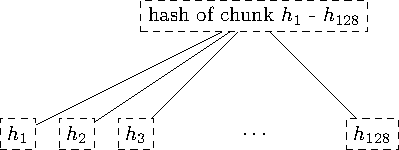
\includegraphics{fig/treebasic.pdf} % requires the graphicx package
   \caption{ A generic node in the tree has 128 children.}
   \label{fig:treebasic}
\end{figure}

During normal swarm lookups, a swarm client performs a lookup for a hash value and receives a chunk in return. This chunk in turn constitutes another $b$ hashes to be looked up and retrieve another $b$ chunks and so on until the chunks received belong to the actual document (see figure \ref{fig:tree2}).


\begin{figure}[htbp]
   \centering
   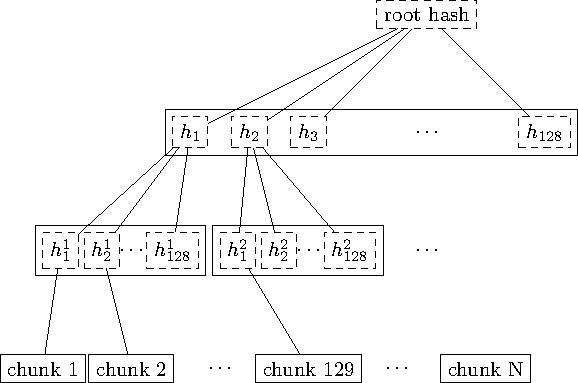
\includegraphics{fig/tree2.pdf} % requires the graphicx package
   \caption{ The swarm tree is the data structure encoding how a document is split into chunks.}
   \label{fig:tree2}
\end{figure}

While off-the-shelf erasure coding could be used on documents uploaded in swarm, this solution has immediate problems. Apart from the quadratic complexity of encoding, chunking the CRS-encoded datablob with the chunker would result in certain chunks being more vulnerable, since their retrieval is dependent on the retrieval of the chunks that encode all their ancestor nodes in the chunktree.

This prompted us to try and align the notion of swarm chunk with the chunk used in the CRS scheme. This led us to encode redundancy directly into the swarm tree by applying the \emph{CRS scheme}  to each set of chunks that are children of a node in the swarm tree.

The \emph{chunker} algorithm using CRS coding works the following way when splitting the document:

\begin{enumerate}
\item Set input to the data blob.
\item Read the input one chunk (say fixed 4096 bytes) at a time. Count the chunks by incrementing a counter $i$. 
\item Repeat 2 until either there's no more data (note: the last chunk read may be shorter) or $i \equiv 0$ mod $m$
\item use the CRS scheme on the last $i \mod\ m$ chunks to produce $k$ parity chunks resulting in a total of $n \leq m+k$ chunks.
\item Calculate the hashes of all these chunks and concatenate them to result in the next chunk (of size $i\mod m$ of the next level. Record this chunk as the next.
\item If there is more data repeat 2. 
\item If there is no more data but the next level data blob has more than one chunk, set the input to this and repeat from 2.
\item Otherwise remember the blob as the root chunk.
\end{enumerate}

% Fixing the branching factor of the swarm hash as $n=128$ and $h=32$ as the size of the \emph{SHA3 Keccak hash} gives us a chunk size of $4096$ bytes.

% We start splitting the input data into chunks, and after each $m$ chunks add $k=n-m$ parity check chunks using a Reed-Solomon code so that now any $m\text{-out-of-}n$ chunks are
% sufficient to reconstruct the document. On the next level up the chunks are composed of the hashes of the $m$  data chunks and the $k$ hashes of the parity chunks. Let's take the first $m$
% of these and add an additional $k$ parity chunks to those such that any $m$ of the resulting $n$
% chunks are sufficient to reconstruct the origial $m$ chunks. And so on and on every level. In terms of
% availability, every subtree is equally important to every other subtree at this level. The resulting
% data structure is not a balanced tree since on every level $i$ the last $k$ chunks are parity leaf
% chunks while the first $m$ are branching nodes encoding a subtree of depth $i-1$ redundantly.
A typical piece of our tree would look like this (see figure \ref{fig:tree-with-erasure}).


\begin{figure}[htbp]
   \centering
   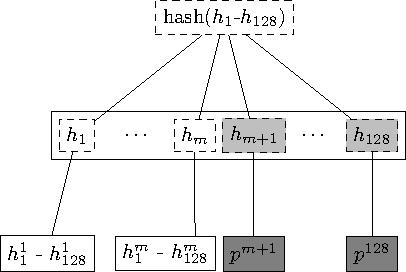
\includegraphics{fig/tree-with-erasure.pdf} % requires the graphicx package
   \caption{The swarm tree with extra parity chunks using $m$ out of 128 CRS code. Chunks $p^{m+1}$ through $p^{128}$ are parity data for chunks $h^1_1 - h^1_{128}$ through $h^{m}_1  - h^{m}_{128}$.}
   \label{fig:tree-with-erasure}
\end{figure}


This pattern repeats itself all the way down the tree. Thus hashes $h^1_{m+1}$ through $h^1_{128}$ point to parity data for chunks pointed to by $h^1_1$ through $h^1_{m}$.Parity chunks $p^i$ do not have children and so the tree structure does not have uniform depth.

If the number of file chunks is not divisible by $m$, we cannot proceed with the last batch in the same way as the others. We propose that we encode the remaining chunks with an erasure code that guarantees at least the same level of security as the others. Note that it is not as simple as choosing the same redundancy. For example a 50-of-100 encoding is much more secure against loss than a 1-of-2 encoding even though the redundancy is 100\% in both cases. Overcompensating, we require the same number of parity chunks even when there are fewer than $m$ data chunks.

This leaves us with only one corner case: it is not possible to use our $m\text{-out-of-}n$ scheme on a single chunk ($m=1$) because it would amount to $k+1$ copies of the same chunk. The problem is that any number of copies of the same chunk all have the same hash and therefore are automatically deduplicated. Thus when there is only a single chunk left over at some level of the tree, we'd have to apply some transformation to it to obtain a second (but different) copy before we could generate more parity chunks.

Whenever a single chunk is left over ($m=1$) (this is always the case for the root chunk itself), we propose to append an extra padding byte to the chunk not counting towards its size. Since the subtree size determines exactly what span of the chunk is substantive data, the  differential padding byte is easily ignored when the document is assembled.%
%
\footnote{%
Note that the typical values for $k$ will be in the single digits so a single byte will always suffice. Note that in the special corner case when the singleton leftover chunk is a full chunk, we end up having an oversized chunk.
}

\subsubsection{Improving efficiency of retrieval with erasure codes}

This per-level $m\text{-out-of-}n$ Cauchy-Reed-Solomon erasure code does not only provide resilience through improved redundancy, but also offers more efficient retrieval in terms of latency\cite{ethersphere2016sw3}.
The systemic code means that the pattern transparently preserves the random-access property of the chunk tree. 
When reading an erasure coded intermediate chunk, there are two possible modes of operation: the cheap method tries to assemble the first $m$ datachunks analogous to the non-erasure coded case, the only difference is that the chunker behaves like the intermediate chunk was $m*h$ long encoding only $m$ chunks of the next level down. 

The other, more expensive, method initiates the retrieval of all $m+k$ chunks. After the first $m$ chunks out of $m+k$ arrive, we use the CRS decoder to reconstruct the data corresponding to the $m$ chunks. Such a race can improve the robustness of retrieval since it hides potentially simultaneous retrieval errors of up to $k$ requests. It also mitigates network throughput restrictions or network connection problems by ignoring the $k$ out of $m+k$ slowest deliveries.

\subsection{Gateways and light nodes}
\label{sec:light}

Light client nodes refer to a special mode of operation necessitated by  poor bandwidth environments, e.g., mobile devices on low throughput networks.

Apart from special treatment of light nodes as kademlia peers, light client nodes become one by virtue of using light node requests. Light server nodes on the other hand are nodes offering to serve light node requests. Stable storage nodes will by default allow light node requests and earn money for their services.

In light mode of operation API calls (download, upload, random access with range queries, domain resolution via ENS, path resolution via manifests) fall back to higher level requests that are sent to light server nodes making the experience similar to using a gateway.

To its peers, a light mode node is revealed implicitly by the node not advertising itself as storer or caching node.
As a consequence, light nodes are not synced to and from, do not expect to serve retrieve requests, and therefore do not count towards saturation in a node's kademlia bin.
Note that otherwise light nodes may participate in real-time message passing services like PSS and therefore their inclusion in the same kademlia table is justified.

Light nodes connect with a few (possibly only one) proxy nodes.
In case the number of light client nodes vs server nodes at one time is too high, we may end up saturating the connectivity of light server nodes. To mitigate this,
we allow streaming protocol over pss relayed by more node types other than light servers.
Therefore we do not require a light node proxy peer to be a light server node as long as it can forward pss requests (they are closer to the target light server or allow universal forwarding in pss).

Once we can assume that light nodes communicate with light servers using the streamer protocol (over rlpx directly or via pss relayed through pss forwarder nodes), we can spell out the light node request types:

Live chunk retrieve requests are handled by an autoregistered pair of streamers, they are responded to with hash checkback if wanted (use-case is racing mode of balancing). Retrieve requests are available to light nodes.

\subsubsection{Light section request}

A remote section request provides provable random access to a document outsourcing to the server peer (1) domain resolution via ENS, (2) path traversal via manifests (not currently provable) (3) random access from range queries. 
Remote section read is for one time lookups in a db or very large resources.
The request contains a swarm url with a range, the result is a corresponding stream of data  with proof.

\subsubsection{Light download}

Light download requests offer an efficient integrity protected read into a file by downloading level one stream (hashes of datachunks) then do a section read just requesting chunks directly. Full resource downloads are self proving, at the end server peer just provides the root hash and client can verify this by calculating the swarm hash of the data stream.
This works best for repeated read at calls (a song, movie) or buffering. Downloads can resume and continue through client restart using the persisted intervals for history syncing. Collection downloads just break down to multiple full downloads. Multiple full downloads can be load balanced over several proxy peers. 

\subsubsection{Light upload}

Client can upload an entire resource to one peer. Non-light nodes will use this request to obtain insurance over a file. 





\cite{ethersphere2016sw3}
\cite{ethersphere2016smash}
\cite{maymounkov2002kademlia}
\cite{heep2010r}
\cite{malavolta2017concurrency}
\cite{chiesa2017decentralized}
\cite{heilman2016tumblebit}
\cite{green2016bolt}
\cite{miller2017sprites}
\cite{mcdonald2017payment}
\cite{diferrante2017payment}

\bibliography{./refs.bib}
% \appendix
% \section{}
\printglossary

\end{document}
